\section{Results and Discussion\label{sec:TC-results}}

\Cref{subfig:TC-res_DV_y} shows that the maximal averaged voltage difference 
$\DV_{y}$ for the \Dtwo~particle while having the leaser in the 
$P_{\text{measure}}$ mode. It has the same shape as the stationary force 
measurement in \cref{subfig:TC-F_y}.  However, the smoothness of $\DV_{y}$ is 
worse. We attribute this to the nature of the experiment, as the recorded 
motion of the particle is caused by two effects; one is the acoustic field and 
the other is the always present Brownian motion.  For the stationary force 
measurements the particle is fixed in place by the optical potential and the 
Brownian motion is negligible.

By measuring the same shape with the two experiments, we could validate our 
measurement protocol. As for the stationary measurements, the SNR of the 
evolution measurement and also shape are better for the in-plane $\ey$ than the 
axial $\ez$ (see \cref{subfig:TC-F_y} and \cref{subfig:TC-F_z}). Nevertheless, 
\cref{subfig:TC-F_z} and \cref{subfig:TC-res_DV_z} also show similar shapes. We 
want to stress again, that the amplitudes of \cref{fig:TC-DV_vs_dy} are not 
comparable to each other for $\ey$ and $\ez$ (see 
\cref{sec:TC-experimental-setup}).
% This step enables data comparability, because the raw magnitudes are 
% inherently different. As stated before, the in-plane position detection along 
% $\ex$ and $\ey$ functions differently than the axial along $\ez$.

The numerical streaming simulations of a fluid cavity with and without the
surrounding structure showed that the streaming field is a local effect in a
model with surrounding structure. In our experiments we saw similar tendencies.  
However, not all measured spatial locations had enough actual signal strength 
to further investigate. In \Cref{fig:TC-evolutioin-V} we plot the time evolution 
of the signal for four different $\Dy$ where it is clear that the signal is due 
to the acoustic field and not to noise or Brownian motion.

\begin{figure}[ht]
  \centering
  \begin{subfigure}{\figWidth}
    \centering
    \caption{Data for $y$-component ($m = y$)}\label{subfig:TC-res_DV_y}
    % \tikzsetnextfilename{avgV_y_vs_dy}
\begin{tikzpicture}
  \begin{axis}[%
      scale only axis,
      width = 60mm,
      height = 45mm,
      xticklabel style={
        /pgf/number format/fixed,
        /pgf/number format/precision=2
      },
      legend style={
        fill=lightgray,
        font=\tiny,
        at={(0.97,0.05)},
        anchor=south east
      },
      legend cell align={left},
      ylabel={$\max\left( \DV_{m}\left( t \right) \right)$ [\si{\mV}]},
      xlabel = {$\Dy$ [\si{\mm}]}]

      \fill[fill=black!15!white] ({axis cs:-0.065,-0.0002}|-{rel axis cs:0,0}) 
      rectangle ({axis cs:-0.025,0.0002}|-{rel axis cs:0,1});

    \addplot[thick,mark=*,mark size=1pt] table[x=dy, y=DV_y_m10] 
    {\relPath/10_Figures/TikZ/averaged_yz_mVoltages.dat};
    \addlegendentry{$\Dz = -10$};

    \addplot[thick, dotted,mark=*,mark size=1pt] table[x=dy, y=DV_y_m00] 
    {\relPath/10_Figures/TikZ/averaged_yz_mVoltages.dat};
    \addlegendentry{$\Dz = 0$};

    \addplot[thick, dashed,mark=*,mark size=1pt] table[x=dy, y=DV_y_p10] 
    {\relPath/10_Figures/TikZ/averaged_yz_mVoltages.dat};
    \addlegendentry{$\Dz = +10$};

    % wavelength
    \draw[|<->|] ({axis cs:-0.135,0}|-{rel axis cs:0,0.55}) -- ({axis 
    cs:0.05,0}|-{rel axis cs:0,0.55}) node[midway,above] 
    {$\sfrac{\lap}{2}=\laF$};

  \end{axis}
\end{tikzpicture}

    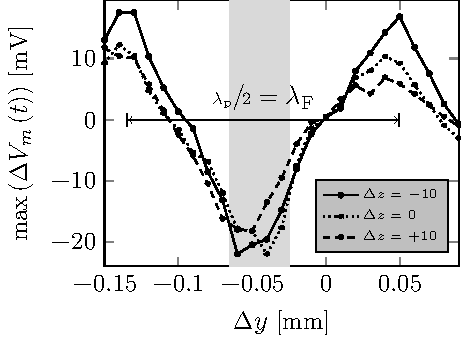
\includegraphics[]{/avgV_y_vs_dy.pdf}
  \end{subfigure}%
  \begin{subfigure}{\figWidth}
    \centering
    \caption{Data for $z$-component ($m = z$)}\label{subfig:TC-res_DV_z}
    % \tikzsetnextfilename{avgV_z_vs_dy}
\begin{tikzpicture}
  \begin{axis}[%
      scale only axis,
      width = 60mm,
      height = 45mm,
      xticklabel style={
        /pgf/number format/fixed,
        /pgf/number format/precision=2
      },
      legend style={
        fill=lightgray,
        font=\tiny,
        at={(0.97,0.05)},
        anchor=south east
      },
      legend cell align={left},
      xlabel = {$\Dy$ [\si{\mm}]}]

      \fill[fill=black!15!white] ({axis cs:-0.065,-0.0002}|-{rel axis cs:0,0}) 
      rectangle ({axis cs:-0.025,0.0002}|-{rel axis cs:0,1});

    \addplot[thick,mark=*,mark size=1pt] table[x=dy, y=DV_z_m10] 
    {\relPath/10_Figures/TikZ/averaged_yz_mVoltages.dat};
    \addlegendentry{$\Dz = -10$};

    \addplot[thick, dotted,mark=*,mark size=1pt] table[x=dy, y=DV_z_m00] 
    {\relPath/10_Figures/TikZ/averaged_yz_mVoltages.dat};
    \addlegendentry{$\Dz = 0$};

    \addplot[thick, dashed,mark=*,mark size=1pt] table[x=dy, y=DV_z_p10] 
    {\relPath/10_Figures/TikZ/averaged_yz_mVoltages.dat};
    \addlegendentry{$\Dz = +10$};

  \end{axis}
\end{tikzpicture}

    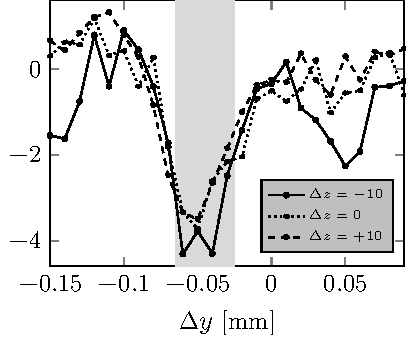
\includegraphics[]{/avgV_z_vs_dy.pdf}
  \end{subfigure}%
  \caption{Maximal $\DV_{y}$ and $\DV_{z}$ averaged over all repetitions in the 
    timespan between \SI{35}{\ms} and \SI{55}{\ms} for the three different 
    measurement heights $\Dz = \SIlist[list-units=single, list-final-separator 
    = {, }, list-pair-separator= {, }] {-10;0;10}{\um}$. The gray shaded area 
    represents the $\Dy_{i}$ of best signal strength for $\max\left( 
    \DV_{z}\left( t \right) \right)$. The data points of best strength are 
    taken for the time evolution results. The wavelength marker represents the 
  same length as in \cref{subfig:TC-F_y}.}\label{fig:TC-DV_vs_dy}
\end{figure}%

Since we show $\DV_{m}$ rather than the absolute voltage amplitudes, we can 
further validate our protocol. For $\sfrac{t}{t_{0}} < 0$, where $t_{0} = 
\sfrac{1}{\fex}$ and $\sfrac{t}{t_{0}}=0$ represents the time when the US is 
switched on (in \cref{fig:TC-daq-sync} $t = \SI{0}{\ms}$), all data series in 
\cref{fig:TC-evolutioin-V} are zero. All data series for $\ez$ are more noisy than 
for $\ey$. However, we also have the same amplitude of noise in $\ey$ 
direction. But, the normalization value for the data series for $\ey$ is 
inherently larger than for $\ez$ (see \cref{fig:TC-DV_vs_dy}).

\afterpage{
\begin{figure}[ht]
  \centering
  % \tikzsetnextfilename{evolution_V}
%%%%%%%
% READ TABLE
%%%%%%%
\pgfplotstableread{\relPath/10_Figures/TikZ/evolution_yz_Voltages.dat}{\data}
%%%%%%%
% LINES FOR ALL GROUPPLOTS
%%%%%%%
\renewcommand{\tikzHelper}{
  \fill[fill=black!10!white] (axis cs:-80,0) rectangle (axis cs:0,1);

  \draw[dotted] (axis cs:0,0) -- (axis cs:0,1);
  \draw[dotted] (axis cs:50,0) -- (axis cs:50,1);
  \draw[dotted] (axis cs:100,0) -- (axis cs:100,1);
  \draw[dotted] (axis cs:-80,0.5) -- (axis cs:120,0.5);
  \draw[dotted] (axis cs:-80,0.5) -- (axis cs:120,0.5);
}



\begin{tikzpicture}
   \begin{groupplot}[%
       scale only axis,
       group style={
         group size= 2 by 4,
         group name=plots,
         vertical sep=4pt,%
         horizontal sep=8pt},%
       height=40mm,%
       width=64mm,%
        xticklabel style={
          /pgf/number format/fixed,
          /pgf/number format/precision=2
        }]

%%%%%%
%%% PLOT (1,1)
%%%%%%

   \nextgroupplot[%
      legend style={
        fill=lightgray,
        font=\tiny,
        at={(0.03,0.95)},
        anchor=north west
      },
      legend cell align={left},
     xticklabels={,,},
     % title={$\DV_{y}\,|\,\Dy = \SI{-0.06}{\milli\meter}$},%
     title={Data for $y$-component ($m = y$)},%
     ylabel={$\sfrac{\DV_{m}}{\DV_{m,\text{max}}}$}]

      \tikzHelper
      \draw[thick,|<->|] (axis cs:-80,0.25) -- (axis cs:0,0.25) node[midway, 
      above] {US off};

      \addplot[thick] table[x=dt, y=DV_y_m06_m10] {\data};

      \addplot[thick, dotted] table[x=dt, y=DV_y_m06_m00] {\data};

      \addplot[thick, dashed] table[x=dt, y=DV_y_m06_p10] {\data};

      \addlegendentry{$\Dz = \SI{-10}{\um}$};
      \addlegendentry{$\Dz = \SI{0}{\um}$};
      \addlegendentry{$\Dz = \SI{+10}{\um}$};



%%%%%%
%%% PLOT (1,2)
%%%%%%

   \nextgroupplot[%
     xticklabels={,,},
     yticklabels={,,},
     title={Data for $z$-component ($m = z$)}]%
   % title={$\DV_{z}\,|\,\Dy = \SI{-0.06}{\milli\meter}$}]

      \tikzHelper

      \addplot[thick] table[x=dt, y=DV_z_m06_m10] {\data};

      \addplot[thick, dotted] table[x=dt, y=DV_z_m06_m00] {\data};

      \addplot[thick, dashed] table[x=dt, y=DV_z_m06_p10] {\data};

%%%%%%
%%% PLOT (2,1)
%%%%%%

   \nextgroupplot[%
     xticklabels={,,},
     ylabel={$\sfrac{\DV_{m}}{\DV_{m,\text{max}}}$ },
     % title={$\Dy = \SI{-0.05}{\milli\meter}$}
   ]

      \tikzHelper

      \addplot[thick] table[x=dt, y=DV_y_m05_m10] {\data};

      \addplot[thick, dotted] table[x=dt, y=DV_y_m05_m00] {\data};

      \addplot[thick, dashed] table[x=dt, y=DV_y_m05_p10] {\data};

%%%%%%
%%% PLOT (2,2)
%%%%%%

   \nextgroupplot[%
     xticklabels={,,},
     yticklabels={,,},
     % title={$\Dy = \SI{-0.05}{\milli\meter}$}
   ]

      \tikzHelper

      \addplot[thick] table[x=dt, y=DV_z_m05_m10] {\data};

      \addplot[thick, dotted] table[x=dt, y=DV_z_m05_m00] {\data};

      \addplot[thick, dashed] table[x=dt, y=DV_z_m05_p10] {\data};

%%%%%%
%%% PLOT (3,1)
%%%%%%

   \nextgroupplot[%
     xticklabels={,,},
     ylabel={$\sfrac{\DV_{m}}{\DV_{m,\text{max}}}$ },
     % title={$\Dy = \SI{-0.04}{\milli\meter}$}
   ]

      \tikzHelper

      \addplot[thick] table[x=dt, y=DV_y_m04_m10] {\data};

      \addplot[thick, dotted] table[x=dt, y=DV_y_m04_m00] {\data};

      \addplot[thick, dashed] table[x=dt, y=DV_y_m04_p10] {\data};

%%%%%%
%%% PLOT (3,2)
%%%%%%

   \nextgroupplot[%
     xticklabels={,,},
     yticklabels={,,},
     % title={$\Dy = \SI{-0.04}{\milli\meter}$}
   ]

      \tikzHelper

      \addplot[thick] table[x=dt, y=DV_z_m04_m10] {\data};

      \addplot[thick, dotted] table[x=dt, y=DV_z_m04_m00] {\data};

      \addplot[thick, dashed] table[x=dt, y=DV_z_m04_p10] {\data};


%%%%%%
%%% PLOT (4,1)
%%%%%%

   \nextgroupplot[%
     ylabel={$\sfrac{\DV_{m}}{\DV_{m,\text{max}}}$},
     xlabel={$10^{3}\,\sfrac{t}{t_{0}}$ },
     % title={$\Dy = \SI{-0.03}{\milli\meter}$}
   ]

      \tikzHelper

      \addplot[thick] table[x=dt, y=DV_y_m03_m10] {\data};

      \addplot[thick, dotted] table[x=dt, y=DV_y_m03_m00] {\data};

      \addplot[thick, dashed] table[x=dt, y=DV_y_m03_p10] {\data};

%%%%%%
%%% PLOT (4,2)
%%%%%%

   \nextgroupplot[%
     yticklabels={,,},
     xlabel={$10^{3}\,\sfrac{t}{t_{0}}$},
     % title={$\Dy = \SI{-0.03}{\milli\meter}$}
   ]

      \tikzHelper

      \addplot[thick] table[x=dt, y=DV_z_m03_m10] {\data};

      \addplot[thick, dotted] table[x=dt, y=DV_z_m03_m00] {\data};

  \end{groupplot}

%%%%%%
%%% TEXT NEXT TO PLOTS
%%%%%%
  \node[rotate=90] at (plots c2r1.east) [yshift=-5mm] {$\Dy = 
  \SI{-0.06}{\milli\meter}$};
  \node[rotate=90] at (plots c2r2.east) [yshift=-5mm] {$\Dy = 
  \SI{-0.05}{\milli\meter}$};
  \node[rotate=90] at (plots c2r3.east) [yshift=-5mm] {$\Dy = 
  \SI{-0.04}{\milli\meter}$};
  \node[rotate=90] at (plots c2r4.east) [yshift=-5mm] {$\Dy = 
  \SI{-0.03}{\milli\meter}$};

\end{tikzpicture}

  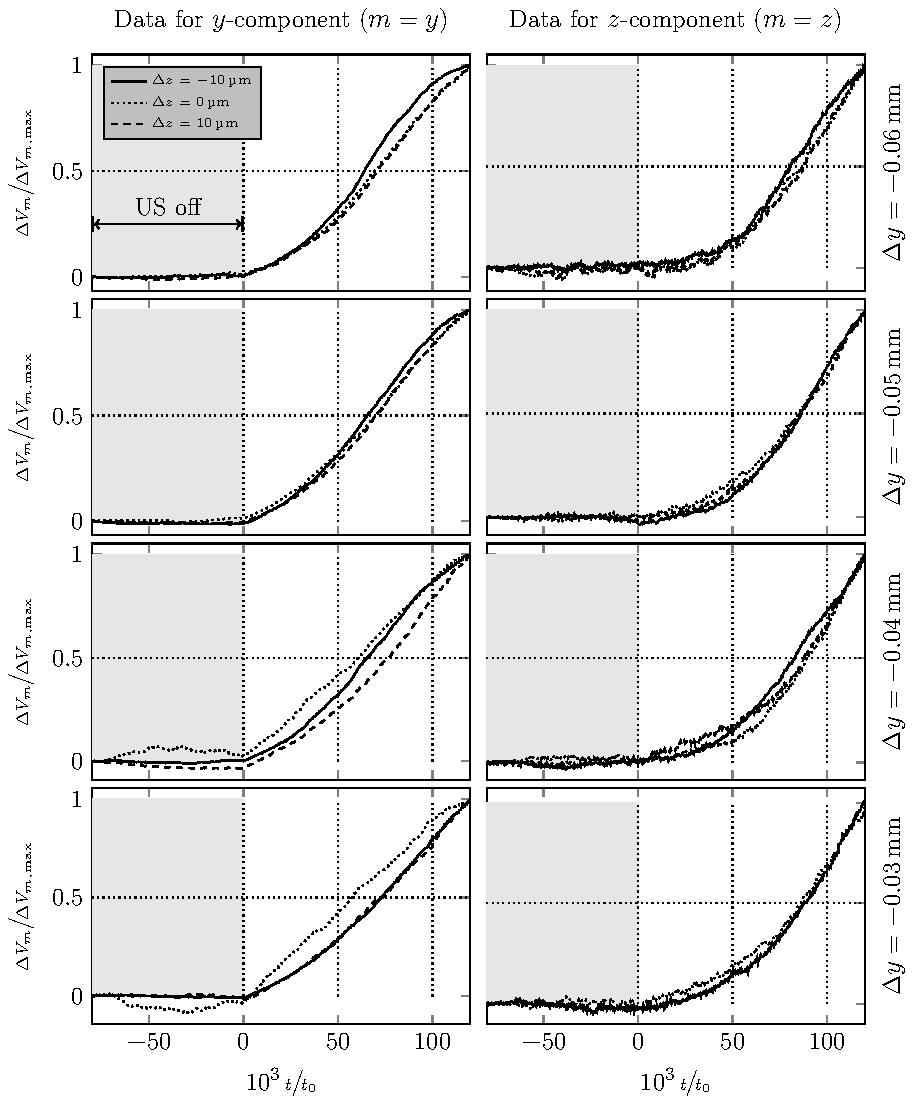
\includegraphics[]{/evolution_V.pdf}
  \caption{Time evolution of the normalized $\DV_{y}$ (left column) and 
    $\DV_{z}$ (right column) for the three measurement heights $\Dz = 
    \SIlist[list-units=single, list-final-separator = {, }, 
    list-pair-separator= {, }] {-10;0;10}{\um}$ and the positions for $\Dy = 
    \SIlist[list-units=single, list-final-separator = {, }, 
    list-pair-separator= {, }] {-0.06;-0.05;-0.04;-0.03}{\mm}$. The gray shaded 
    area of each plot marks the time when the US is off; 
  $t_{0}=\sfrac{1}{\fex}$.}\label{fig:TC-evolutioin-V}
\end{figure}
}

For all 12 positions $(y_{i}, z_{j})$ in \cref{fig:TC-evolutioin-V} the signal 
along $\ey$ starts changing as soon as the US is switched on. This 
is in line with the estimation of \cref{eq:TC-tau-arf} for $\tarf$. For all data 
series $m = z$ it takes significantly more time until the movement with 
constant velocity starts. To further compare the results, we take as criteria 
the period $p^{\ast} = \sfrac{t^{\ast}}{t_{0}}$, when the normalized $\DV_{m} 
\ge 0.5$ is reached. In \cref{tab:TC-results}, the absolute periods for this 
criteria and the offset between the movement along $\ey$ ($m=z$) and the 
movement along $\ez$ ($m=y$) are shown. Taking a different criteria value 
(e.g., the normalized $\DV_{m} \ge 0.3$) changes the absolute magnitude of the 
values $p^{\ast}$, however the offset does not change significantly. The 
average for all $\Delta p^{\ast}$ is about 17'500 which equates to $\approx 
\SI{4.35}{\ms}$ for the excitation frequency $\fex = \SI{4.015}{\MHz}$.

\begin{table*}
  \centering
  \footnotesize
  \begin{tabular}{ll *{4}{x{27mm}}}
    \toprule
    \toprule
  {\bfseries $\Dy$} & [\si{\mm}] & -0.06 & -0.05 & -0.04 & -0.03 \\

    \midrule
    % {\small
  {\bfseries $p^{\ast}_{y}$ } & ($\times 1000$) [-] & 64.2, 69.5, 70.7 & 65.8, 
  70.3, 70.3 & 65.8, 60.6, 76.7 & 73.5, 57.4, 74.3 \\[2mm]

  {\bfseries $p^{\ast}_{z}$} & ($\times 1000$) [-] & 80.7, 87.9 88.3 & 86.3, 
  85.5, 86.7 & 83.1, 89.5, 87.5 & 87.9, 86.7,  \\

    \midrule
    
  {\bfseries $\Delta p^{\ast}$} & ($\times 1000$) [-] & 16.5, 18.4, 17.6 & 
  20.5, 15.2, 16.4 & 17.3, 18.9, 10.8 & 14.4, 29.3, \\
    % }
    \bottomrule
    \bottomrule
    
  \end{tabular}
  \caption{Absolute periods $p^{\ast}_{m}$ when the normalized $\DV_{m} > 0.5$.  
    The three values per column correspond to the three heights $\Dz = 
    \SIlist[list-units=single, list-final-separator = {, }, 
    list-pair-separator= {, }] {-10;0;10}{\um}$ per $\Dy$ respectively. For 
  $\Dy = \SI{-0.03}{\mm}$ and $\Dz = \SI{10}{\um}$ no data is available for 
$p_{z}^{\ast}$. The last row states the offset $\Delta p^{\ast} = p^{\ast}_{z} 
- p^{\ast}_{y}$}\label{tab:TC-results}
\end{table*}

In addition, all slopes for the $y$ movement ($m=y$) are linear almost 
immediately after the US is
switched on. This suggests, that the ARF is constant and accelerates the 
particle fast to its terminal velocity. The measured voltages and also their 
differences are linearly related to the traveled distances. Hence, a constant 
increase in voltage, which means a constant voltage increase per time 
$\sfrac{\text{d}\,\DV_{m}}{\text{d}t} = const.$, implies a constant particle 
speed along the $\ey$ direction. The particle trajectory in $\ez$ direction is 
predominantly affected by the streaming field. This fluid motion takes more 
time until it is established. With the same reasoning as before, a linear slope 
for the $z$ movement ($m=z$) in \cref{fig:TC-evolutioin-V} implies a constant 
force and constant particle speed. A constant speed means a non-changing 
streaming field and therefore a constant streaming velocity.

